\documentclass[sigconf,nonacm]{acmart}

% links
\usepackage{hyperref}
% foreach macro
\usepackage{pgffor}
% file contents utilities
\usepackage{filecontents}

\usepackage{array}

\usepackage{subcaption}

%%
%% \BibTeX command to typeset BibTeX logo in the docs
\AtBeginDocument{%
  \providecommand\BibTeX{{%
    \normalfont B\kern-0.5em{\scshape i\kern-0.25em b}\kern-0.8em\TeX}}}

\newcolumntype{L}{>{\centering\arraybackslash}m{3cm}}

\begin{document}

%%
%% The "title" command has an optional parameter,
%% allowing the author to define a "short title" to be used in page headers.
\title{Coimf \\ Collecting Implicit User Feedback for \\ WordPress Websites}

%%
%% The "author" command and its associated commands are used to define
%% the authors and their affiliations.
%% Of note is the shared affiliation of the first two authors, and the
%% "authornote" and "authornotemark" commands
%% used to denote shared contribution to the research.
\author{Adrian David Castro Tenemaya}
\email{adrian.castro@tum.de}
\affiliation{%
  \institution{Technische Universit{\"a}t M{\"u}nchen}
}

%%
%% The abstract is a short summary of the work to be presented in the
%% article.
\begin{abstract}
  Recommender Systems (RS) are one of the most impactful ways that an
  online company can generate revenue from. They empower the final users by
  offering personalized recommendations based on their interests and interaction
  with a service. Collecting this kind of information however is not trivial.
  There are two ways that an RS uses in order to make such suggestions: explicit
  feedback and implicit feedback. The first refers to feedback that the user
  is giving the system explicitly, either by assigning a range of numeric values
  to a certain item, or by using a binary system to like or dislike it. This
  kind of feedback however requires a certain amount of effort from the user,
  which is not always possible to have. Instead, implicit feedback can be used
  to infer users interests, without interfering with its experience.

  State-of-the-art algorithms for recommender systems that uses implicit
  feedback are being developed using popular datasets such as Adressa
  \footnote{\href{http://reclab.idi.ntnu.no/dataset/}{http://reclab.idi.ntnu.no/dataset/}}
  and MovieLens
  \footnote{\href{https://grouplens.org/datasets/movielens/}{https://grouplens.org/datasets/movielens/}},
  and most of the available ones have limited language availability.

  In this work, we will explore the implementation of Coimf, a WordPress plugin
  that collects implicit user feedback such as navigation, click and reading
  behavior. The goal is to create a framework that can be used by recommender systems
  to generate recommendations for news articles and e-commerce products
  based on user implicit feedback.
\end{abstract}


%%
%% The code below is generated by the tool at http://dl.acm.org/ccs.cfm.
%% Please copy and paste the code instead of the example below.
%%
\begin{CCSXML}
  <ccs2012>
  <concept>
  <concept_id>10002951.10003317.10003331</concept_id>
  <concept_desc>Information systems~Users and interactive retrieval</concept_desc>
  <concept_significance>500</concept_significance>
  </concept>
  </ccs2012>
\end{CCSXML}

\ccsdesc[500]{Information systems~Users and interactive retrieval}

%%
%% Keywords. The author(s) should pick words that accurately describe
%% the work being presented. Separate the keywords with commas.
\keywords{datasets, recommender system, behavior tracking, navigation behavior}

%%
%% This command processes the author and affiliation and title
%% information and builds the first part of the formatted document.
\maketitle

\section{Introduction}

Across the years a class of methods called ``Recommender Systems'' (RS) have been
developed to accommodate the increasing necessity to aid users in navigating items,
in situations where they can be overloaded with information, and cannot simply
explore every simple option.
RS work by trying to predict how much a user is likely to appreciate a list of items,
and ranking them accordingly. A user can express how much they like something either
by explicitly telling the system how much they like an item using a given scale (1 to 5,
1 to 7, 1 to 10, etc...), or by implicit means, like the time of navigation,
or by how many times they play a song for example.

Explicit feedback from the user is the most accurate amongst the two previous ways,
and it is widely used across many services, like e-commerce, recipe
websites, online movies streaming platforms and more. However, this kind of feedback
is also the most difficult to gather, as this requires an effort from the user side,
and is usually scarce because of this.

Implicit feedback on the other hand is much more abundant, as it does not require much
effort (if at all) from the user, and can be collected much more easily.
Over the years new and more efficient methods to gather this data have been
developed. However, because the collection of implicit feedback generates tons
of data, is also very noisy, and can often be misleading.

There exist three macro types of algorithms used by most recommender
systems.

\textbf{Content Based Filtering} analyses every item and how
a user rates it and builds a model tailored to the specific user \cite{ricci2011}.

\textbf{Collaborative Filtering} on the other hand builds a model for an item
using multiple ratings from multiple users for the single item \cite{ricci2011}.

\textbf{Hybrid Filtering} uses a combination of two or more recommendation
algorithms \cite{burke2002hybrid}.

The underlying algorithm being used amongst most commercial applications nowadays
is collaborative filtering \cite{Koren2011}. However, there are some problems with
this approach \cite{ilievski2013}. Collaborative filtering systems has been
proved to work very well in scenarios where the number of items do not often
vary \cite{huang2007comparison}, and are also always relevant over time. On the
other hand, news blogs have a concept of ``freshness'', where an article
published one hour ago is much more relevant than the same type of content
published one month, or even one year ago. Recommending a user something
``fresh'' will make the user trust the recommender system, as they will see that
the recommendations are not just taken from the ``top-10'' items in a category,
but are actually relevant in time and space. For example, recommending the
latest New York news to someone who lives in California is not great, and so is
recommending something from 6 months ago, which may contain plain wrong information.

Implicit feedback datasets available online like \cite{wumind, gulla2017adressa} are
of good quality and of decent size, but the availability for multiple languages
is very limited, or completely absent. With this in mind, we developed Coimf
(Collect Implicit Feedback), a WordPress plugin that allows blogs and e-commerce
owners to collect and generate their own implicit feedback dataset, regardless
of the language.

During the development of Coimf, a series of test and changes were made by
observing the live results on Tuttobarche, a popular Italian WordPress boating
blog.

We will briefly describe previous work, our implementation, the challenges of the
process, and future proceedings of the work.

\section{Related Work}
\label{sec:related-work}

The approach illustrated by Google on their work from 2010 \cite{liu2010personalized}
is a good example on how implicit user feedback can be successfully used to generate
on the fly quality user recommendations. The work uses United States
click data from their Google News website to create users interest profiles and
clicks. It is important to note that not only user interests are gathered,
but also local news trends, as the combination of the two can express a change in
a user's interest over particular events (Beijing 2008 for example saw a huge spike
in sports search queries). In this work, users are also location-bounded, in order
to have a better definition of what users search for in a specific area.
Interests are then combined and fed into a Bayesian framework
\cite{nielsen2009bayesian, rendle2012bpr}
for user interests, and then they obtain a prediction for the user's current
news interest. A list of articles is then calculated by combining
a score for each article using content-based filtering \cite{van2000using}
and a collaborative filtering score. The conclusion of the work is that a hybrid
recommender system which uses both content-based filtering and implicit feedback
is possible, and in this case increased user trust for the recommender system,
as they slowly started using more the recommendation section than the regular,
non-personalized one.

An approach for collaborative filtering using implicit feedback data is illustrated
on \cite{hu2008collaborative}, and shows the challenges of dealing with implicit
feedback. This work uses a model that assigns an estimation user-item to whether
the user ``likes'' or ``dislikes'' an item, and has the interesting feature to
scale with input size. Along with recommendations, the proposed model is also
able to provide explanations for them, which is something that tries to address the
open problem for explainable recommendations \cite{zhang2014explicit,
  zhang2018explainable}.

An effort to understand if implicit feedback data can be useful for e-commerce
recommendation systems has been done on work \cite{peska2012estimating}. After
collecting data about different types of user-generated events, they proceeded
to test recommender systems to use first one kind of implicit feedback at a
time, and then combining them to make recommendations. The combination part
proved to be successful. As stated on the paper however, more search is needed,
as the significance of these improvements is not very high, and is most likely
due to the low amount of data available to the authors.

\subsection{Popular Implicit Feedback Datasets}

A popular dataset for news recommender system called Adressa was released on 2017
\cite{gulla2017adressa}. It consists of 20M entries from a 10-week period and a
smaller dataset of 2M entries from a 1-week period. It has been used over the
last three years to build news recommender systems. The data collected offers a
very good starting point for building an implicit feedback dataset, which is
amongst the final goals of this work.

A relatively new dataset called \textbf{MIND} (\textbf{Mi}crosoft \textbf{N}ews
\textbf{D}ataset) \cite{wumind} has been released around April 2020, and uses
data from Microsoft News website, in English. In the paper, some news
recommender algorithms
\footnote{\href{https://github.com/microsoft/recommenders}{https://github.com/microsoft/recommenders}}
are used to evaluate the quality of the data, with excellent results.

\subsection{Explicit Feedback Datasets}

Even though the following datasets consists of explicit feedback, we will include
them anyways, as often in literature the explicit ratings are ``converted'' to
implicit feedback \cite{feigl2018neural, manzato2013gsvd, hidasi2012fast}.

The \textbf{Movielens} dataset is vastly known and popular in literature, as it has been
used ever since its publication in 1998. Back then, it consisted of just around
100K user ratings, but now a version of 25M user ratings is available.

The \textbf{Netflix} dataset
\footnote{\href{https://www.kaggle.com/netflix-inc/netflix-prize-data}{https://www.kaggle.com/netflix-inc/netflix-prize-data}}
was made available from Netflix in 2006 for the famous ``Netflix Prize'', which
offered 1M dollars for the best collaborative filtering algorithm to predict
user ratings for movies. They gave people access to a huge amount of data about
movie ratings, around 100M user ratings by 480K users on 17K movies. Numerous
papers used this dataset as a base to build their own collaborative filtering
algorithms, but the limitation is that it consists of only explicit feedback.

\section{Framework Overview}

Coimf (Collect Implicit Feedback) is the name of the plugin that was developed to
tackle the task of collecting implicit feedback data from users of blogs.
We decided to develop Coimf for WordPress because as of today, it is
the most stable and widespread software used for the creation of blogs and
e-commerce, both areas where the collection and understanding of implicit
feedback data can have a meaningful impact on the proceedings of the area.

Online blogs with hundreds or thousands of articles such as news websites, often
rely solely on simple and uncomplicated ways to target users with more articles,
such as ``if you have read this article, you might like this one from the same category'',
or ``read more articles from the same author'', or by simply recommending a fixed
set of articles chosen by the editors.

The goal of \textit{Coimf} is to be a framework to collect implicit user
feedback, which in turn can be used to feed a recommender system. This has the
advantage to be independent of the local language it is implemented in, which is
a huge drawback of current datasets.

WordPress itself offers a solid framework that give us useful information about
the content being consumed. For example, no data about how many words there are
in an article will be recorded by Coimf, as we can very easily extract this
information from WordPress.

\subsection{Data Storage}

Because we are using WordPress as a base, Coimf uses the built-in methods to
access read and write operations on the database. For simplicity, the current
structure is made of just one table \\ \texttt{wp\_coimf\_Actions} shown in Table~\ref{tbl:data-structure}.

\begin{table}[h]
  \centering

  \begin{tabular}{ | c | c | L | }
    \hline
    Name                  & Type     & Description                                 \\ \hline
    \texttt{user\_id}     & BIGINT   & Identifier of a visiting user               \\ \hline
    \texttt{session\_id}  & BIGINT   & Identifier of a generated web session       \\ \hline
    \texttt{id}           & ULONG    & Action identifier                           \\ \hline
    \texttt{action\_type} & UINT8    & Type of the action (0 = page view, 1 = page
    click, 2 = page read)                                                          \\ \hline
    \texttt{time\_start}  & DATETIME & When the action started                     \\ \hline
    \texttt{time\_end}    & DATETIME & When the action ended                       \\ \hline
    \texttt{value}        & LONGTEXT & JSON-encoded data about the action          \\ \hline
  \end{tabular}

  \caption{Data structure}
  \label{tbl:data-structure}
\end{table}

Ideally, the structure should be split into the different number of
tracked actions, so that we wouldn't need to parse the JSON-encoded data every
time, which can be expensive when taking very large amounts of data into
account, but a temporary solution was made to accommodate a faster development.

All \texttt{DATETIME} entries in the database are stored in UTC time.

What follows is a list of each user action and how it's encoded into the
database.

\begin{itemize}
  \item \textbf{Page View Action}: the action saves two variables, \texttt{from} and
        \texttt{to}: the first encodes where the user was before they landed on the
        latter.
  \item \textbf{Page Click Action}: when a user clicks on a web page, the mouse coordinates
        within that page is logged as \texttt{mouseX} and \texttt{mouseY}, along with
        the screen resolution, \texttt{resolutionX} and \texttt{resolutionY}, the user
        is currently using.
  \item \textbf{Page Read Action}: when a user reaches a particular point in a page, we
        assume that the user has ``read'' the page (e.g. when they reach the bottom of
        an article). We log the page location on \texttt{location} and how long did it
        took for the user to reach that point with \texttt{pageTime}.
\end{itemize}

\subsection{Administrator Area}

In a normal scenario, a regular user visiting the website wouldn't be able to
take a look at the collected data. Only users with special Administrator
permissions should be able to access it. WordPress offers us with the ability to
do just that, by having a dedicated administrator area where we can create and
set up a page dedicated to Coimf and its settings. For this subsection, we will
use the term ``user'' to indicate a user with administrator permissions.

To date, Coimf has four active pages:

\textbf{Data}: the user can browse the data collected so far, order it by time and
action type.

\textbf{Read Time Visualizations}: the user can see different visualizations of
the page read times of the last week.

\textbf{Session Visualizations}: the user is shown a series of graphs indicating
regarding web sessions of the last week.

\textbf{Settings}: it is possible to customize different aspects of Coimf in
this area, like the reading minimum and maximum times, the tracked pages and
where the user has to scroll in order to count as a page read action.

\subsection{Cookies and Privacy Concerns}

Coimf uses cookies to track users as they are using the website. Cookies are necessary
to understand whether a user is new to the website or is a returning visitor, and they
are store in the user's device for a period of at most one week since its last visit.
If users do not return after one week has passed, cookies are automatically deleted
from their device.

The user has to specifically opt-in when navigating WordPress for cookies to be
stored in his device.

\subsection{Web Session}

First, we have to find the first event that initiates a session
\cite{liu2010personalized, gulla2017adressa}. Every
subsequent within 30 minutes of the last event is considered part of the current
\textit{web session}.

A \textit{web session} can contain events like page views, clicks, e-commerce
transactions and more. A \textit{web session} ends when thirty (30) minutes have
passed since the last user interaction. This is because when a user leaves the website for more than this amount of time,
we can safely assume that their current query and research has been satisfied,
and the next time he returns he will not (most likely) look for the same things
in the same way as the previous session. Time of the day, his geographical
location can change and interfere heavily on a user's navigation choice. An
example of a user session can be seen on Figure~\ref{fig:web-session-example},
where the same user can create multiple sessions, if separated by at least 30
minutes of activity.

\begin{figure}[h]
  \centering
  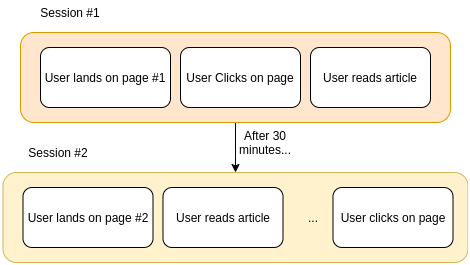
\includegraphics[width=\linewidth]{session-example.png}
  \caption{Web Session Example}
  \Description[Web Session Example]{Web Session Example}
  \label{fig:web-session-example}
\end{figure}

An effort to understand whether a user is actively looking at a web page
has been done before \cite{kim2005implicit}, but the use of a camera that scans
a user's motion and face position is not really feasible, and would require a
user's camera access permission.

\subsection{Tracked User Behavior}

Arguably, everything that a user interacts with and the time it takes for him to
do so can be interpreted as an implicit feedback. The challenge is to understand
what signals are useful, and how to interpret them correctly to make useful and
thoughtful predictions. Early categorizations of user behavior can be found in
\cite{nichols1998implicit, Oard1998ImplicitFF}. Tracked metrics have been chosen
following the user interaction categories denoted in \cite{lerche2016using},
in Table ~\ref{tbl:selected-user-behavior}.
\begin{table}[h]
  \centering

  \begin{tabular}{ | cp{0.5 \linewidth} | cp{\linewidth} }
    \hline
    Category                & Tracked Observable Behavior                         \\ \hline
    Examination             & Duration of viewing time, duration of reading time,
    selection of text parts, repeated consumption, page clicks                    \\
    Social \& Public Action & Public Posting, Commenting and Communicating        \\
    \hline
  \end{tabular}

  \caption{Selected User Behavior}
  \label{tbl:selected-user-behavior}
\end{table}

These categories of user behavior were selected for their simplicity and for
making a proof of concept of the functionality of Coimf.

\subsection{Navigation Data}

Most (if not all) users landing on a website come from a source that is not the
same as the website where Coimf is used. Because of this, we also track where
the traffic is coming from, also known as the referrer.

It is possible however, that some entries do not contain a starting referrer at all. This can be due to a lot of
factors, but if the user navigates from an internal web page to another internal
web page, the referrer (source location) is always present.

It is possible to transform the data gathered in this way into a directed
graph $G = (v, e)$ where $v$ is the list of collected nodes (the pages that were
navigated), and $e \subseteq \{ (x, y) | (x, y) \in v^2 \land x \neq y \}$
(source and destination locations are different, as noted in
section~\ref{sec:challenges}).

\subsection{Read Time}

Read time is often used in literature \cite{hu2008collaborative, liu2010personalized, chaturvedi2017}
as a way to understand a user's interest on a certain topic, or an article's freshness.
After seven days of tracking, we can see the distribution on Figure
~\ref{fig:page-read-times-dist} of read time across all articles on Tuttobarche,
with an indication that most users (\~85-90\%) do not read for more than 200 seconds,
or 3 minutes.
The threshold of maximum reading time before a user is considered away from keyboard,
and thus not interesting for our data, is set to one hour, or 3600 seconds. This
setting can be adjusted, but it can skew the data if non-rank based correlation
measures are used. An interesting approach on the problem to track user
activity described on \cite{chaturvedi2017} was to track user scroll wheel, page
up-down, and the times the user scrolled on the page. This can be used as an
additional metric to understand if the current user is actively reading the
page, or just forgot about it when it was reading, thus generating an entry in
our dataset in the far-end of the distribution for read times.

\subsection{Click Data}
\label{sec:click-data}

Along with the data mentioned above, also clicks are being collected.
Specifically, coordinates on the web page and the screen resolution of the
device is being logged.

At first, this seemed to be a nice compromise, as the first thought was to be
able to dynamically create screenshots for every logged resolution, and then
place the clicks on top of it to create a Heatmap of where user clicks the most.
However, this revealed to be a bad strategy, as there are so many combinations
of different resolutions that the solution above is infeasible, and inaccurate.
To date, we collected 253 different resolutions. Because of this, we will not
include the logged data on Section~\ref{sec:experiments-and-data-analysis}.

As noted on \cite{kim2005implicit} however, mouse move and mouse clicks are very
good indicators that can help us understand the level of engagement of a user on
a web page. For example, if the user has clicked on an article or item, but is
not moving the mouse at all, maybe he has gone for a break, closed the tab or
misclicked. All indicators of the fact that the user was \textbf{not interested}.

\section{Challenges of Implicit Feedback Collection}
\label{sec:challenges}

Because of the noisy and uncertain nature of implicit feedback, it is not a
trivial task to put in place a set of rules to lower the uncertainty of the results.

For example, when a user visits a website page, they can simply leave it open and take a
coffee break for ten or more minutes, thus leaving us to guess whether this user
is either a very slow reader or very interested in the page.

Because of this, there are inevitably some challenges that arise from the
implementation of a tracking system.
For example, Coimf cannot reliably track a user's behavior across multiple
devices without an authentication system active at all times, such as Google.

A naïve approach would be to use a single IP address to identify a single
user and its multiple devices, but this approach does not take into account that
more physical users can use the same IP address, for example a home or an office.
Also using the GPS position of a user is something that is not viable, as it raises
privacy concerns, and more often than not is unreliable to understand whether
the user is alone or with other people. This approach is also as accurate as the GPS
system that the user has installed in its device (if any), which is not super high,
even by today's standards.

Some filtering on the incoming data has been done in order to avoid noise:

\textbf{Bots}: Traffic coming from bots (such as crawlers) has been excluded, as they are not
considered as traffic coming from users.

\textbf{Page Refreshes}: The same criteria have been applied to traffic
coming from page refreshes (excluding source and destination link which are equal),

\textbf{Asynchronous Requests}: Async requests and \textit{cron jobs}, as these
are not traffic coming from a user interaction.

\textbf{Administrators}: Navigation data from users with administration or publisher
permissions is also not being logged.

\textbf{Special Paths}: certain WordPress directories and locations, such as
``/wp-login'', ``/wp-admin'', ``/wp-includes'' and ``/wp-cron.php'', are also
excluded from the tracking, as these are locations that a user is not allowed to
access under regular navigation conditions, and do not contain any recommendable
item.

\section{Experiments and Data Analysis}
\label{sec:experiments-and-data-analysis}

The selected approach proved to be successful at capturing data from user navigation.
So far, the system has gathered more than 147.000 user actions within a 7 days time span,
gathering on average around 19.000 unique user actions a day on Tuttobarche.

The data collected is automatically fed into graphs generated using the famous
JavaScript library D3.js. This allows us to focus on the collection of the data
rather than its visualization, which is also not the focus of this work.

From 08 June to 14 June, data has been collected using Coimf on the whole news
section Tuttobarche, and the results are shown on Table~\ref{tbl:data-collected-statistics}.

\begin{table}[h]
  \centering
  \caption{Statistics of collected data}

  \begin{subtable}{\linewidth}
    \caption{Count of logged actions}
    \begin{tabular}{ | L | L | }
      \hline
      Action Type & Count            \\ \hline
      Page View   & \texttt{129.000} \\ \hline
      Page Click  & \texttt{9.500}   \\ \hline
      Page Read   & \texttt{8.600}   \\ \hline
      Total       & \texttt{147.100} \\ \hline
    \end{tabular}
  \end{subtable}
  \begin{subtable}{\linewidth}
    \caption{Average Per Day}
    \begin{tabular}{ | L | L | }
      \hline
      Action Type    & Average          \\ \hline
      Page View      & \texttt{\~18500} \\ \hline
      Page Click     & \texttt{\~1400}  \\ \hline
      Page Read Time & \texttt{\~96s}   \\ \hline
    \end{tabular}
  \end{subtable}

  \label{tbl:data-collected-statistics}
\end{table}

\subsection{Navigation Data}

An example of a typical user navigation can be seen on Figure~\ref{fig:user-navigation-graph}, where we can see a
user's first arrival and his actions through time.

In this case, a user first lands on WordPress landing page (``/magazine/''),
navigates onto a page where a list of boat trials are shown, and looks for a
specific keyword. He then proceeds to navigate to an article that showcases a
boat trial (``Bayliner 742 Cuddy'') and finishes reading the article in about
one minute and a half.

\begin{figure}[h]
  \centering
  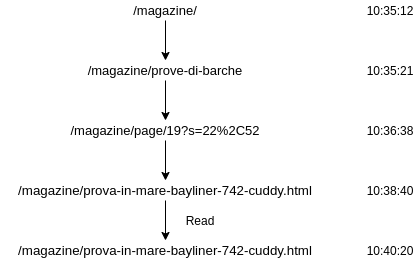
\includegraphics[width=\linewidth]{Directed_Graph.png}
  \Description[User Navigation Graph]{User Navigation Graph}
  \caption{User Navigation Graph}
  \label{fig:user-navigation-graph}
\end{figure}

It is also possible to obtain taxonomy data from each path, thanks
again to WordPress core, which enables us to query the current path and obtain
the post metadata. The post metadata includes things like the title, the category,
the article contents and so on.

Taxonomy data is of course useful as noted by Section~\ref{sec:related-work} to
understand user's current interests, and their interest over time.

\subsection{Read Time}

As Figure~\ref{fig:page-read-times-dist} suggest, user read times are in the
first part of the distribution.

\begin{figure}[h]
  \centering
  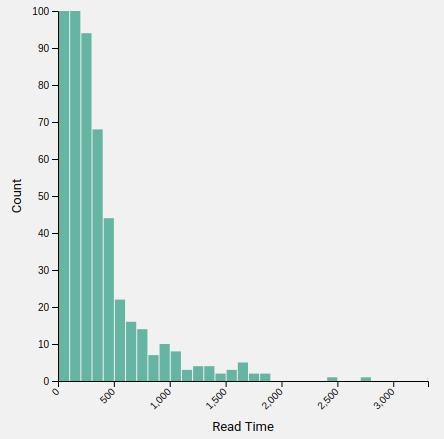
\includegraphics[width=0.8 \linewidth]{page-read-time-distribution.png}
  \Description[Distribution of page read times]{Distribution of page read times}
  \caption{Distribution of page read times of the last 7 days on Tuttobarche}
  \label{fig:page-read-times-dist}
\end{figure}

Also, Figure~\ref{fig:page-read-times-dist-dense} shows that most users reaching the end
of the article within 10 seconds. However, we can also note some spikes around
100 seconds and 170 seconds, which are the estimated reading time for a
Tuttobarche article.

\begin{figure}[h]
  \centering
  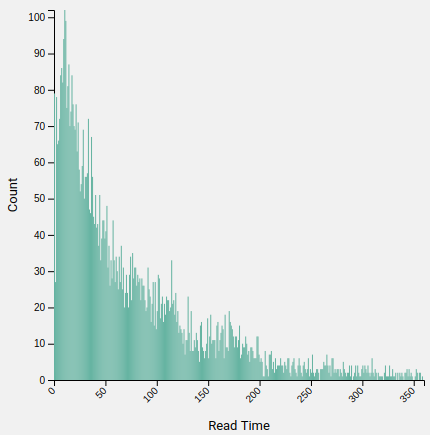
\includegraphics[width=0.8 \linewidth]{page-read-time-distribution-dense.png}
  \Description[Distribution of page read times]{Distribution of page read times}
  \caption{Distribution of page read times up to 6 minutes of the last 7 days on Tuttobarche}
  \label{fig:page-read-times-dist-dense}
\end{figure}

\subsection{Activity Data}
\label{sec:activity-data}

In Figure~\ref{fig:session-heatmap} the data of one week of user activity on
Tuttobarche reveals a lot about the development and the kind of users that are
navigating the website. We can see for example that some changes to the data
collection were made on 11 June, and as a result, we caught more sessions that
were not accounted for before the change. We can also detect behavioral patterns
around noon and night, whilst activity is at its lowest after midnight.

\begin{figure}[h]
  \centering
  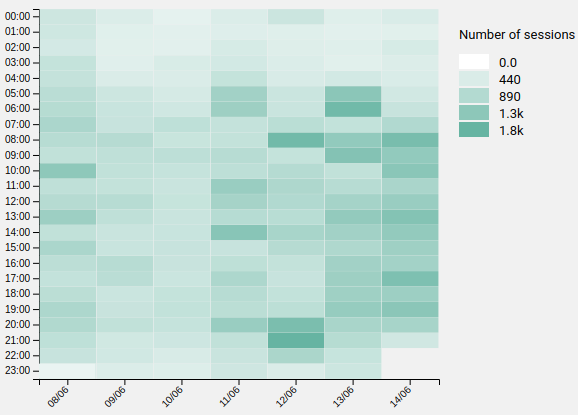
\includegraphics[width=0.8 \linewidth]{session-heatmap.png}
  \Description[Heatmap of active sessions over 7 days]{Heatmap of active sessions over 7 days}
  \caption{Heatmap of sessions over 7 days on Tuttobarche}
  \label{fig:session-heatmap}
\end{figure}

This data can be adjusted to show when articles are read the most, and when it
is the best time to post an article for it to be successful. Recommender systems
can also use this information to rank an article or item based on user activity
and ``freshness''.

\section{Conclusion}

Implicit feedback is much more abundant and easy to collect than explicit feedback.
However, the large and noisy amount of data coming from the first method leads to
more challenges. Which user actions are useful, and which are just plain noise,
and should not be taken into account are all aspects that should not be taken
lightly. This is particularly important as highlighted on
Section~\ref{sec:activity-data}, because ignoring user activity can lead to an
underestimation of active sessions and the data collected.

Coimf will help WordPress based websites to build an implicit feedback dataset
of their own, from scratch, without having to develop dedicated solutions 

The insights gathered with Coimf are also being used to power marketing operations
on Tuttobarche, which further highlights the potential of this work not only as
a framework for recommender systems, but also as a powerful marketing tool.

\section{Future Work}

To date, companies have few tools available to them to collect implicit feedback
data. There is also a very small selection of publicly available frameworks, like
Implicit
\footnote{\href{https://implicit.readthedocs.io/}{https://implicit.readthedocs.io/}}
and Surprise \footnote{\href{http://surpriselib.com}{http://surpriselib.com}},
that use implicit data to make recommendations. One improvement that can be done
to \textit{Coimf} is to be able to output data in a format acceptable for the two
frameworks mentioned above.
We believe that the development and nurturing of Coimf can be of huge impact to
the community, and will hopefully enable more users to come up with novel ideas
in the area.

After a first evaluation of the framework and a solid code review, it would be
possible to use the data generated from this framework to build a recommender
system could be the next step. Because WordPress is used as the base, it should
be fairly simple to have a high rate of adoption amongst websites that want to
experiment and give feedback about possible improvements. Furthermore, it is
very important that the data being collected using this means is suitable to be
made open source, as one problem in literature is reproducibility and the
availability of training data for machine learning applications \cite{joachims2017accurately}.

A better solution for the problem presented in Section~\ref{sec:click-data}
would be to log the query selector for the item that has been clicked. This
would allow to have a more precise understanding of which exact element a user
clicked on, thus allowing us to dynamically generate a screenshot with a more
diverse range of resolutions.

Adding the functionality for the framework to establish a ``freshness'' metric
to every article would be a plus, so that recommender systems that uses this
kind of information can make useful recommendations based on when an article was
posted, and for how long it has been relevant for the audience.

Implementing an integration for the famous plugin ``WooCommerce'' could also be
a parallel step. A lot of small companies rely solely on simple methods of data
tracking, and enabling these users with a more powerful, open source tool can
impact the quality of life of many.

Detaching the project from its WordPress implementation and transforming it to a
self-contained framework can be the next step for enabling non-WordPress users to use and start
a recommender system of their own, hence helping the further development of this field.

%%
%% The next two lines define the bibliography style to be used, and
%% the bibliography file.
\bibliographystyle{ACM-Reference-Format}
\bibliography{seminar}

%%
%% If your work has an appendix, this is the place to put it.
\appendix

\section{Online Resources}
The source code of this paper's work is licensed under GPL v3 and can be found at
the following link:

\href{https://github.com/IAL32/wordpress-collect-implicit-feedback}{https://github.com/IAL32/wordpress-collect-implicit-feedback}.

\end{document}
\endinput
